% This file was created with tikzplotlib v0.10.1.
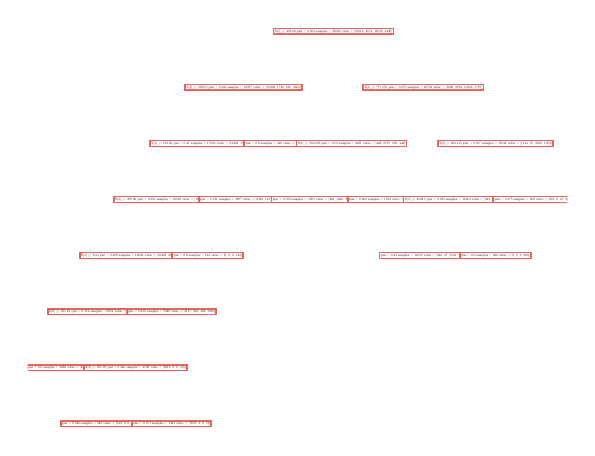
\begin{tikzpicture}

\definecolor{darkgray176}{RGB}{176,176,176}
\definecolor{tomato2369992}{RGB}{236,99,92}

\begin{axis}[
hide x axis,
hide y axis,
tick align=outside,
tick pos=left,
x grid style={darkgray176},
xmin=0, xmax=1,
xtick style={color=black},
y grid style={darkgray176},
ymin=0, ymax=1,
ytick style={color=black}
]
\draw (axis cs:0.133333333333333,0.0625) node[
  scale=0.121348494600586,
  fill=white,
  draw=tomato2369992,
  line width=0.6pt,
  inner sep=3.6pt,
  text=black,
  rotate=0.0,
  align=center
]{gini = 0.346
samples = 648
value = [144, 0, 0, 504]};
\draw (axis cs:0.266666666666667,0.0625) node[
  scale=0.121348494600586,
  fill=white,
  draw=tomato2369992,
  line width=0.6pt,
  inner sep=3.6pt,
  text=black,
  rotate=0.0,
  align=center
]{gini = 0.071
samples = 1944
value = [1872, 0, 0, 72]};
\draw (axis cs:0.0666666666666667,0.1875) node[
  scale=0.121348494600586,
  fill=white,
  draw=tomato2369992,
  line width=0.6pt,
  inner sep=3.6pt,
  text=black,
  rotate=0.0,
  align=center
]{gini = 0.0
samples = 4262
value = [4262, 0, 0, 0]};
\draw (axis cs:0.2,0.1875) node[
  scale=0.121348494600586,
  fill=white,
  draw=tomato2369992,
  line width=0.6pt,
  inner sep=3.6pt,
  text=black,
  rotate=0.0,
  align=center
]{X[2] <= 505.99
gini = 0.346
samples = 2592
value = [2016, 0, 0, 576]};
\draw (axis cs:0.133333333333333,0.3125) node[
  scale=0.121348494600586,
  fill=white,
  draw=tomato2369992,
  line width=0.6pt,
  inner sep=3.6pt,
  text=black,
  rotate=0.0,
  align=center
]{X[0] <= 295.23
gini = 0.154
samples = 6854
value = [6278, 0, 0, 576]};
\draw (axis cs:0.266666666666667,0.3125) node[
  scale=0.121348494600586,
  fill=white,
  draw=tomato2369992,
  line width=0.6pt,
  inner sep=3.6pt,
  text=black,
  rotate=0.0,
  align=center
]{gini = 0.458
samples = 5840
value = [4147, 263, 402, 1028]};
\draw (axis cs:0.2,0.4375) node[
  scale=0.121348494600586,
  fill=white,
  draw=tomato2369992,
  line width=0.6pt,
  inner sep=3.6pt,
  text=black,
  rotate=0.0,
  align=center
]{X[1] <= 2.62
gini = 0.308
samples = 12694
value = [10425, 263, 402, 1604]};
\draw (axis cs:0.333333333333333,0.4375) node[
  scale=0.121348494600586,
  fill=white,
  draw=tomato2369992,
  line width=0.6pt,
  inner sep=3.6pt,
  text=black,
  rotate=0.0,
  align=center
]{gini = 0.0
samples = 144
value = [0, 0, 0, 144]};
\draw (axis cs:0.733333333333333,0.4375) node[
  scale=0.121348494600586,
  fill=white,
  draw=tomato2369992,
  line width=0.6pt,
  inner sep=3.6pt,
  text=black,
  rotate=0.0,
  align=center
]{gini = 0.32
samples = 11658
value = [943, 67, 9501, 1147]};
\draw (axis cs:0.866666666666667,0.4375) node[
  scale=0.121348494600586,
  fill=white,
  draw=tomato2369992,
  line width=0.6pt,
  inner sep=3.6pt,
  text=black,
  rotate=0.0,
  align=center
]{gini = 0.0
samples = 206
value = [0, 0, 0, 206]};
\draw (axis cs:0.266666666666667,0.5625) node[
  scale=0.121348494600586,
  fill=white,
  draw=tomato2369992,
  line width=0.6pt,
  inner sep=3.6pt,
  text=black,
  rotate=0.0,
  align=center
]{X[0] <= 298.06
gini = 0.321
samples = 12838
value = [10425, 263, 402, 1748]};
\draw (axis cs:0.4,0.5625) node[
  scale=0.121348494600586,
  fill=white,
  draw=tomato2369992,
  line width=0.6pt,
  inner sep=3.6pt,
  text=black,
  rotate=0.0,
  align=center
]{gini = 0.551
samples = 4997
value = [2983, 1457, 124, 433]};
\draw (axis cs:0.533333333333333,0.5625) node[
  scale=0.121348494600586,
  fill=white,
  draw=tomato2369992,
  line width=0.6pt,
  inner sep=3.6pt,
  text=black,
  rotate=0.0,
  align=center
]{gini = 0.702
samples = 3059
value = [462, 1246, 907, 444]};
\draw (axis cs:0.666666666666667,0.5625) node[
  scale=0.121348494600586,
  fill=white,
  draw=tomato2369992,
  line width=0.6pt,
  inner sep=3.6pt,
  text=black,
  rotate=0.0,
  align=center
]{gini = 0.062
samples = 1592
value = [0, 1541, 51, 0]};
\draw (axis cs:0.8,0.5625) node[
  scale=0.121348494600586,
  fill=white,
  draw=tomato2369992,
  line width=0.6pt,
  inner sep=3.6pt,
  text=black,
  rotate=0.0,
  align=center
]{X[5] <= 2502.5
gini = 0.339
samples = 11864
value = [943, 67, 9501, 1353]};
\draw (axis cs:0.933333333333333,0.5625) node[
  scale=0.121348494600586,
  fill=white,
  draw=tomato2369992,
  line width=0.6pt,
  inner sep=3.6pt,
  text=black,
  rotate=0.0,
  align=center
]{gini = 0.375
samples = 268
value = [201, 0, 67, 0]};
\draw (axis cs:0.333333333333333,0.6875) node[
  scale=0.121348494600586,
  fill=white,
  draw=tomato2369992,
  line width=0.6pt,
  inner sep=3.6pt,
  text=black,
  rotate=0.0,
  align=center
]{X[1] <= 138.23
gini = 0.41
samples = 17835
value = [13408, 1720, 526, 2181]};
\draw (axis cs:0.466666666666667,0.6875) node[
  scale=0.121348494600586,
  fill=white,
  draw=tomato2369992,
  line width=0.6pt,
  inner sep=3.6pt,
  text=black,
  rotate=0.0,
  align=center
]{gini = 0.0
samples = 422
value = [0, 0, 0, 422]};
\draw (axis cs:0.6,0.6875) node[
  scale=0.121348494600586,
  fill=white,
  draw=tomato2369992,
  line width=0.6pt,
  inner sep=3.6pt,
  text=black,
  rotate=0.0,
  align=center
]{X[1] <= 583.805
gini = 0.58
samples = 4651
value = [462, 2787, 958, 444]};
\draw (axis cs:0.866666666666667,0.6875) node[
  scale=0.121348494600586,
  fill=white,
  draw=tomato2369992,
  line width=0.6pt,
  inner sep=3.6pt,
  text=black,
  rotate=0.0,
  align=center
]{X[2] <= 203.115
gini = 0.357
samples = 12132
value = [1144, 67, 9568, 1353]};
\draw (axis cs:0.4,0.8125) node[
  scale=0.121348494600586,
  fill=white,
  draw=tomato2369992,
  line width=0.6pt,
  inner sep=3.6pt,
  text=black,
  rotate=0.0,
  align=center
]{X[5] <= 2502.5
gini = 0.431
samples = 18257
value = [13408, 1720, 526, 2603]};
\draw (axis cs:0.733333333333333,0.8125) node[
  scale=0.121348494600586,
  fill=white,
  draw=tomato2369992,
  line width=0.6pt,
  inner sep=3.6pt,
  text=black,
  rotate=0.0,
  align=center
]{X[1] <= 771.555
gini = 0.557
samples = 16783
value = [1606, 2854, 10526, 1797]};
\draw (axis cs:0.566666666666667,0.9375) node[
  scale=0.121348494600586,
  fill=white,
  draw=tomato2369992,
  line width=0.6pt,
  inner sep=3.6pt,
  text=black,
  rotate=0.0,
  align=center
]{X[1] <= 481.66
gini = 0.684
samples = 35040
value = [15014, 4574, 11052, 4400]};
\end{axis}

\end{tikzpicture}
